\documentclass[12pt]{amsart}
\usepackage{/home/nigel/Dropbox/mystyle}
\usepackage{tikz}
\usetikzlibrary{trees}
\usetikzlibrary{automata, positioning}

\begin{document}

\iffalse
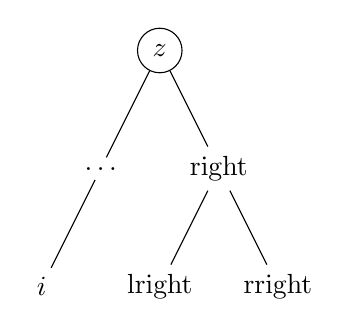
\begin{tikzpicture}
	\node[circle,draw](z){$z$}
		child{node {$\ldots$}
		      child{node {$i$}}
		      child[missing] %child{node {rleft}}
		}
		child{node {right}
		      child{node {lright}}
		      child {node {rright}}
		};
\end{tikzpicture}
\fi

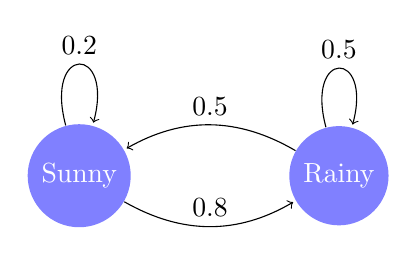
\begin{tikzpicture}

% Add the states
\node[state,
		text=white,
		draw=none,
		fill=white!50!blue] (s) {Sunny};

\node[state,
		right=2cm of s,
		text=white,
		draw=none,
		fill=white!50!blue] (r) {Rainy};

	 \draw[every loop]
	  (s) edge[loop above] node {0.2} (s)
		(s) edge[bend right,auto=left] node {0.8} (r)
		(r) edge[bend right,auto=right] node {0.5} (s)
		(r) edge[loop above] node {0.5} (r);
\end{tikzpicture}

\end{document}
